\begin{frame}
\thetitle{ELBO Objective}

    \begin{align*}
        \argmax_{\theta, \lambda} \ELBO(\theta, \lambda)  &=\argmax_{\theta, \lambda}\sum_{n=1}^{N} \ELBO(\theta, \lambda \param x^{(n)})\\
        &= \argmax_{\theta, \lambda} \sum_{n=1}^N \E_{ q}\Big[\log \frac{p(x^{(n)}, z^{(n)} \param \theta)}{q(z^{(n)} \given x^{(n)} \param \lambda)} \Big] 
    \end{align*}
    \air

% \begin{enumerate}
% \item General case: gradient ascent on ELBO, e.g. VAE, SVI.
% \item Special cases: exploit structure of $p,q$, e.g. EM, CAVI.
% \end{enumerate}
\end{frame}

\begin{frame}
\thetitle{Maximizing ELBO: Model Parameters}
%Maximizing ELBO with respect to $\theta$ is equivalent to maximizing 
%\[\argmax_{\theta}  \E_{q(z;\lambda)} \log p(x, z \param \theta) \]

\[\argmax_{\theta} \textcolor{red}{\E_{q}\Big[\log \frac{p(x, z \param \theta)}{q(z \given x;\lambda)} \Big]} = \argmax_{\theta}  \E_{q} \log p(x, z \param \theta) \]

\air

\begin{center}
\begin{tikzpicture}
    \draw[decorate,decoration={brace,amplitude=10pt}] (-0.3, 0) -- node[xshift=-1cm]{$\alert{\ELBO}$} (-0.3, 2);
    
    \draw[red] (0, 0) rectangle (1, 2);
    %\draw[blue] (0, 2) rectangle (1, 3);
    
    \draw[->] (1.5, 1.5) --node[yshift=0.5cm]{$\theta$} (2.5, 1.5) ; 
    \begin{scope}[xshift = 3cm]
    %\draw[decorate,decoration={brace,amplitude=10pt}] (-0.3, 0) -- node[xshift=-0.75cm]{$$} (-0.3, 3);
    
    \draw[red] (0, 0) rectangle (1, 2.5);
    %\draw[blue] (0, 2.5) rectangle (1, 3);
    \draw[decorate,decoration={brace,amplitude=5pt}] (1.3, 2.5) -- node[xshift=1.2cm]{$\alert{\text{ELBO}}$} (1.3, 0);
    %\draw[decorate,decoration={brace,amplitude=5pt}] (1.3, 3) -- node[xshift=1.5cm]{$\structure{\text{posterior gap}}$} (1.3, 2.5);
\end{scope}
\end{tikzpicture}
\end{center}
Intuition: Maximum likelihood problem under variables drawn from $q(z \given x; \lambda)$. 
\air 

\end{frame}


\begin{frame}
\thetitle{Fitting Model: Gradient Ascent on Model Parameters}
Easy: Gradient respect to $\theta$
\begin{align*}
\nabla_{\theta} \ELBO(\theta, \lambda \param x) &=  \nabla_\theta \E_{ q}\Big[ \log p(x^{}, z^{} \param \theta) \Big] \\
&= \E_{q}\Big[\nabla_{\theta} \log p(x^{}, z^{} \param \theta) \Big] 
\end{align*}
\begin{itemize}
    \item Since $q$ not dependent on $\theta$, $\nabla$ moves inside expectation.
    \item Estimate with samples from $q$. Term $\log p(x, z \param \theta)$ is easy to evaluate. Single sample is often sufficient. 
    \item In special cases, can exactly evaluate expectation.
\end{itemize}
\end{frame}




\begin{frame}
\thetitle{Maximizing ELBO: Variational Distribution }
% Maximizing ELBO with respect to $\lambda$ is equivalent to minimizing $\KL[q(z;\lambda) \Vert p(z \given x \param \theta)]$
% \begin{align*}
%     %\ELBO(\theta, q \param x) &= \log p(x \param \theta) - \KL[q(z) \Vert p(z \given x \param \theta)] \\
%     \argmax_{\lambda} \alert{\ELBO}(\theta, \lambda) &= \argmin_{\lambda} \structure{\KL[q(z;\lambda)\ \Vert\ p(z \given x \param \theta)]} 
% \end{align*}

\vspace{-0.5cm}
\begin{align*}
    \argmax_{\lambda}  &\alert{\ELBO}(\theta, \lambda) \\
    &= \argmax_{\lambda} \log p(x \param \theta) - \textcolor{blue}{\KL[q(z\given x ;\lambda)  \, \Vert \, p(z \given x \param \theta)]} \\
    &= \argmin_{\lambda} \textcolor{blue}{\KL[q(z \given x ;\lambda)\ \Vert\ p(z \given x \param \theta)]}
\end{align*}

% \textcolor{red}{\E_{q(z)}\Big[\log \frac{p(x, z \param \theta)}{q(z;\lambda)} \Big]} + \textcolor{blue}{\KL[q(z;\lambda)  \, \Vert \, p(z \given x \param \theta)]}

\begin{center}
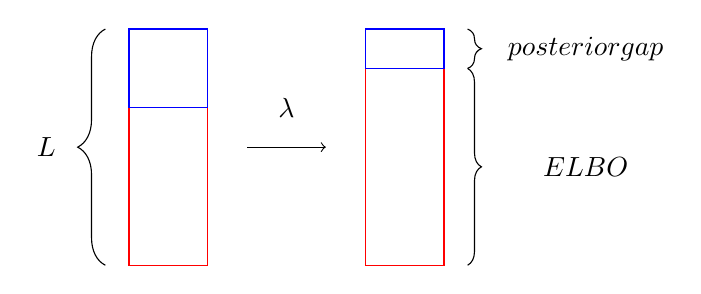
\begin{tikzpicture}
    \draw[decorate,decoration={brace,amplitude=10pt}] (-0.3, 0) -- node[xshift=-0.75cm]{$L$} (-0.3, 3);
    
    \draw[red] (0, 0) rectangle (1, 2);
    \draw[blue] (0, 2) rectangle (1, 3);
    
    \draw[->] (1.5, 1.5) --node[yshift=0.5cm]{$\lambda$ } (2.5, 1.5) ; 
    \begin{scope}[xshift = 3cm]
    %\draw[decorate,decoration={brace,amplitude=10pt}] (-0.3, 0) -- node[xshift=-0.75cm]{$$} (-0.3, 3);
    
    \draw[red] (0, 0) rectangle (1, 2.5);
    \draw[blue] (0, 2.5) rectangle (1, 3);
    \draw[decorate,decoration={brace,amplitude=5pt}] (1.3, 2.5) -- node[xshift=1.5cm]{$\alert{\text{ELBO   }}$} (1.3, 0);
    \draw[decorate,decoration={brace,amplitude=5pt}] (1.3, 3) -- node[xshift=1.5cm]{$\structure{\text{posterior gap}}$} (1.3, 2.5);
\end{scope}
\end{tikzpicture}
\end{center}

Intuition: $q$ should approximate the posterior $p(z |x)$. However, may be difficult if $q$ or $p$ is a deep model.
\air 
%(Note that this optimization is in function space)
\end{frame}

\begin{frame}
\thetitle{Fitting Variational Parameters: Gradient Ascent on $\lambda$?}
Hard: Gradient respect to $\lambda$ 
\begin{align*}
\nabla_{\lambda} \ELBO(\theta, \lambda \param x) &=  \nabla_\lambda \E_{ q}\Big[ \log p(x^{}, z^{} \param \theta) \Big] \\
&\ne \E_{q}\Big[\nabla_{\lambda} \log p(x^{}, z^{} \param \theta) \Big] 
\end{align*}
\begin{itemize}
    \item Cannot naively move $\nabla$ inside the expectation, since  $q$ depends on $\lambda$.
    \item This section: Fitting $\lambda$ in practice:
        \begin{enumerate}
        \item Direct 
        \item Sampling: score function, reparameterization
        \item Conjugacy: closed-form, coordinate ascent
    \end{enumerate}

\end{itemize}
\end{frame}

% \begin{frame}
% \thetitle{General Strategy: Gradient Ascent on ELBO}
% \[ \nabla_{\theta} \ELBO(\theta, \lambda) =  \sum_{n=1}^N  \E_{ q}\Big[\nabla_{\theta} \log p(x^{(n)}, z^{(n)} \param \theta) \Big] \]
% \[ \nabla_{\lambda} \ELBO(\theta, \lambda) =  \nabla_{\lambda} \sum_{n=1}^N  \E_{ q}\Big[ \log \frac{p(x^{(n)}, z^{(n)} \param \theta)}{q(z^{(n)} \given x^{(n)} \param \lambda)} \Big] \]

% First term is easy to calculate via 
% sampling or enumeration (since $\log p(x, z \param \theta)$ is easy). $\nabla_\lambda$ is much harder.
%   \vspace{0.25cm}
 
%  We consider the following strategies:
%     \begin{enumerate}
%         \item Enumeration
%         \item Sampling: score function, reparameterization
%     \end{enumerate}
% \end{frame}

\subsection{Direct}

\begin{frame}
\thetitle{Strategy 1: Direct}
\begin{align*}
 \nabla_{\lambda} \ELBO(\theta, \lambda &\param x^{}) = \nabla_{\lambda} \E_{ q(z \given x^{} \param \lambda)} \Big[ \log \frac{p(x^{}, z \param \theta)}{q(z \given x^{} \param \lambda)} \Big]\\
 & =  \nabla_{\lambda} \Big( \sum_{z \in \mcZ}q(z \given x^{} \param \lambda) \log \frac{p(x^{}, z \param \theta)}{q(z \given x^{} \param \lambda)} \Big)
 \end{align*}

\begin{itemize}
    \item Naive enumeration: Linear in $|\mcZ|$.
    \item Depending on structure of $q$ and $p$, potentially faster with dynamic programming.
    \item Applicable mainly to Model 1 and 3 (Discrete and Structured Models).
\end{itemize}
\end{frame}



\begin{frame}
\thetitle{Example: Model 1 - Naive Bayes}
    \begin{center}

    \begin{tikzpicture}
      %\tikz{
    % nodes
    
     \node[latent] (zl) {$z^{}$};%
     \node[const, below=of zl] (xl) {$x^{}$};%
     \node[const, left=of zl] (lambda) {$\lambda$};
     \edge{lambda}{zl};
     \edge{xl}{zl};
    
    \begin{scope}[xshift=5cm, yshift=-1cm]
    \node (dots) {$\ldots$};%
     \node[obs, left=1cm of dots] (x1) {$x_1^{}$};%
     \node[obs, right=1cm of dots] (xT) {$x_T^{}$};%
     \node[latent, above=5mm of dots] (z) {$z^{}$}; %

     \edge {z} {dots};
     \edge {z} {x1};
     \edge {z} {xT};
     \end{scope}
     \draw (zl) edge[dashed] (z);
     \draw (zl) edge[dashed, bend right=20] (z);
     \draw (zl) edge[dashed, bend left=20] (z);

     \end{tikzpicture}    
     \end{center}
     Let $q(z \given x \param \lambda) = \text{Cat}(\nu)$  where $\nu = \enc(x; \lambda)$  
\begin{align*}
 \nabla_{\lambda} \ELBO(&\theta, \lambda \param x^{}) = \nabla_{\lambda} \E_{ q(z \given x^{} \param \lambda)} \Big[ \log \frac{p(x^{}, z \param \theta)}{q(z \given x^{} \param \lambda)} \Big]\\
 & =  \nabla_{\lambda} \Big( \sum_{z \in \mcZ}q(z \given x^{} \param \lambda) \log \frac{p(x^{}, z \param \theta)}{q(z \given x^{} \param \lambda)} \Big)\\
  & =  \nabla_{\lambda} \Big( \sum_{z \in \mcZ}\nu_z \log \frac{p(x^{}, z \param \theta)}{\nu_z} \Big)
 \\
 %&= \nabla_\lambda \Big( \sum_{k=1}^K  \lambda_k \big( \log \frac{\lambda_k}{\mu_k} +  \sum_{t=1}^T \log f(z \param \theta)_{x_t}\big)\Big)
 \end{align*}
 
     
    %        \[ p(x , z \param \theta) = p(z \given \mu) \prod_{t=1}^T p(x_t \given z \param \theta)\]
    %\begin{enumerate}
    %    \item $z \sim \text{Cat}(\mu)$
    %    \item $x_t \sim \text{Cat}(f(z \param \theta))$
    %\end{enumerate}
\end{frame}

%\begin{frame}
%\thetitle{Strategy 1: Enumeration}
%%Let $q(z \given x \param \lambda) = \text{Cat}(\lambda)$ 
%\begin{align*}
% \nabla_{\lambda} \ELBO(&\theta, \lambda \param x^{}) = \nabla_{\lambda} \E_{ q(z \given x^{} \param \lambda)} \Big[ \log \frac{p(x^{}, z \param \theta)}{q(z \given x^{} \param \lambda)} \Big]\\
% & =  \nabla_{\lambda} \Big( \sum_{z \in \mcZ}q(z \given x^{} \param \lambda) \log \frac{p(x^{}, z \param \theta)}{q(z \given x^{} \param \lambda)} \Big)
% \\
% &= \nabla_\lambda \Big( \sum_{k=1}^K  \lambda_k \big( \log \frac{\lambda_k}{\mu_k} +  \sum_{t=1}^T \log f(z \param \theta)_{x_t}\big)\Big)
% \end{align*}
% (Not the optimal strategy)
%\end{frame}

% \begin{frame}
% \thetitle{Tactic 1b: Dynamic Programming}

% Summary: Sum out structure in $q$. 

% \[ \nabla_{\lambda} \ELBO(\theta, \lambda) =  \sum_{n=1}^N \nabla_{\lambda} \E_{ q(z \param \lambda)}\Big[\log \frac{p(x^{}, z \param \theta)}{q(z;\lambda)} \Big] \]
% \begin{itemize}
%     \item Compute $\nabla_{\lambda} \E_{ q(z \param \lambda)}$ with dynamic programming.
%     \item Applicable only to Model 3 (Structured LVs). Depends on structure
%     \item Note: Can be difficult to implement GPUs. However becoming much easier.  
% \end{itemize}
% \end{frame}


% \begin{frame}
% \thetitle{Example 1b: HMM}
% Run dynamic programming pass (forward algorithm) to compute expectation:

% \[ \nabla_{\lambda} \E_{ q(z_1)}[\log p(z_1) +  \E_{ q(z_2)}[ \log p(z_2 | z_1) +  \E_{q(z_3)} [ \log(z_3 | z_2) \ldots \]
% \begin{itemize}
%     \item Algorithm consists of multiplies and adds (log-semiring). Full differentiable. 
%     \item Similar approach can be used for parsing and tree structures. 
% \end{itemize}
% \end{frame}

% \begin{frame}
% \thetitle{Tactic 2: Sampling}
% Idea: approximate gradient with Monte-Carlo sampling 
% \air 
% Score function gradient estimator.

% \end{frame}
% Naive approach (incorrect):
% \air

% First, sample $\tilde{z}^{(1)} \ldots \tilde{z}^{(J)} \sim q(z;\lambda, x^{})$.
% \air

% Then 
% \begin{align*}
%      \nabla_{\lambda} \ELBO(\theta, \lambda) &=  \sum_{n=1}^N  \nabla_{\lambda} \E_{q(z \param \lambda)} \Big[ \log \frac{p(x^{}, z \param \theta)}{q(z;\lambda)} \Big] \\ 
%     &=\sum_{n=1}^N \frac{1}{J} \sum_{j=1}^J \Big[\nabla_{\lambda} \log \frac{p(x^{}, \tilde{z}^{(j)} \param \theta)}{q(\tilde{z}^{(j)};\lambda)} \Big]
% \end{align*}

% Issue: drops impact of $\lambda$ in expectation.  
% \end{frame}

\subsection{Sampling}


\begin{frame}
\thetitle{Strategy 2: Sampling}
\begin{align*}
    \nabla_\lambda &\ELBO(\theta, \lambda ; x) =  \nabla_\lambda \E_q \Big[\log \frac{\log p(x, z \param \theta)}{\log q (z \given x \param \lambda)} \Big]\\
    &= \nabla_\lambda \alert{\E_{ q}\Big[ \log p(x^{}, z^{} \param \theta) \Big]} -\nabla_\lambda \E_{ q}\Big[ \log q( z^{} \given x^{} \param \theta) \Big]  
\end{align*} 

\begin{itemize}
    \item How can we approximate this gradient with sampling?
    \item Naive monte-carlo fails to provide non-zero gradient.
    \[ z^{(1)}, \dots, z^{(J)} \sim q(z \given x^{} \param \lambda) \]
 \[ \nabla_\lambda \sum_{j=1}^J \Big[ \log p(x^{}, z^{(j)} \param \theta) \Big] = 0\]
    \item Manipulate expression so we can move $\nabla_\lambda$ inside $\E_q$ before sampling.
\end{itemize}
\end{frame}


\begin{frame}
\thetitle{Strategy 2a: Sampling --- Score Function Gradient Estimator}
First term. Use basic identity:

\[\nabla \log q = \frac{\nabla q}{q} \Rightarrow \nabla q  = q \nabla \log q \]

Policy-gradient style training \citep{Williams1992}
\begin{align*}
    \nabla_\lambda & \E_{q}\Big[\log p(x^{}, z \param \theta) \Big] \\
    &=  \sum_z  \log p(x^{}, z \param \theta) \nabla_\lambda   q(z \given x \param \lambda )  \\
        &=  \sum_z  \log p(x^{}, z \param \theta)  q(z \given x \param \lambda )  \nabla_\lambda \log q(z \given x^{} \param \lambda)  \\
    &= \E_{q}\Big[ \log p(x^{}, z \param \theta) \nabla_\lambda \log q(z \given x^{} \param \lambda) \Big]
\end{align*}
\end{frame}

\begin{frame}
\thetitle{Strategy 2a: Sampling --- Score Function Gradient Estimator}
Second term. Need additional identity:
\[\sum \nabla q = \nabla \sum q = \nabla 1 = 0 \]
\vspace{-5mm}
\begin{align*}
    \nabla_\lambda & \E_{q}\Big[\log q(z \given x \param \lambda) \Big] \\
    &= \sum_{z} \nabla_\lambda \Big ( q(z \given x\param \lambda) \log q(z \given x \param \lambda)\Big) \\
    &= \sum_{z}  \log q(z \given x \param \lambda) \nabla_\lambda q(z \given x \param \lambda) +  \frac{q(z \given x \param \lambda)}{q(z \given x \param \lambda)}\nabla_\lambda q(z \given x \param \lambda)\\
    &= \sum_{z}  \log q(z \given x \param \lambda) \nabla_\lambda \log q(z \given x \param \lambda) + \underbrace{\sum_z \nabla_\lambda q(z \given x \param \lambda)}_{= 0} \\
    &= \E_{q}[\log q (z \given x \param \lambda) \nabla_\lambda q (z \given x \param \lambda)]
\end{align*}
\end{frame}

\begin{frame}
\thetitle{Strategy 2a: Sampling --- Score Function Gradient Estimator}
Putting these togther
\begin{align*}
       \nabla_\lambda \ELBO(\theta, \lambda ; x) &=  \nabla_\lambda \E_q \Big[\log \frac{\log p(x, z \param \theta)}{\log q (z \given x \param \lambda)} \Big]\\
       &= \E_q \Big[\log \frac{p(x, z \param \theta)}{q(z \given x \param \lambda)} \nabla_\lambda \log q ( z \given x \param \lambda ) \Big] \\
       &= \E_q \Big[R_{\theta, \lambda}(z) \nabla_\lambda \log q ( z \given x \param \lambda ) \Big]
\end{align*}
\end{frame}

\begin{frame}
\thetitle{Strategy 2a: Sampling --- Score Function Gradient Estimator}
Estimate with samples 
\[ z^{(1)}, \dots, z^{(J)} \sim q(z \given x^{} \param \lambda) \]
\begin{align*}
        \E_{q}&\Big[ R_{\theta, \lambda}(z)  \nabla_\lambda \log q(z \given x^{} \param \lambda) \Big] \\ &\approx \frac{1}{J}\sum_{j=1}^J R_{\theta, \lambda}(z^{(j)})  \nabla_\lambda \log q(z^{(j)} \given x^{} \param \lambda)
\end{align*}
Intuition: if a sample $z^{(j)}$ is has high reward $R_{\theta, \lambda}(z^{(j)})$,
increase the probability of $z^{(j)}$
by moving along the gradient $\nabla_\lambda \log q(z^{(j)} \given x \param \lambda)$.
\end{frame}

\begin{frame}
\thetitle{Strategy 2a: Sampling --- Score Function Gradient Estimator}
\begin{itemize}
    \item Essentially reinforcement learning with reward $R_{\theta, \lambda}(z)$
    \item Unbiased estimator for the gradient, but high variance.
    \item In practice, need variance-reducing \textbf{control variate} $B$.
\end{itemize}    
%     \item Can be estimated with another neural net regressed on the ``reward", e.g.
%     \[ \Big(B(x^{} \param \psi) -  \frac{1}{J}\sum_{j=1}^J \log \frac{p(x^{}, z^{(j)} \param \theta)}{q(z^{(j)} \given x^{} \param \lambda)}\Big)^2 \]
% \end{itemize}
% \begin{align*}
%     &\E_{q(z \given x^{} \param \lambda)}\Big[ \log \frac{p(x^{}, z \param \theta)}{q(z \given x^{} \param \lambda)} \nabla_\lambda \log q(z \given x^{} \param \lambda) \Big]
%     \\ &=     \E_{q(z \given x^{} \param \lambda)}\Big[\Big( \log \frac{p(x^{}, z \param \theta)}{q(z \given x^{} \param \lambda)} - B\Big) \nabla_\lambda \log q(z \given x^{} \param \lambda) \Big]
% \end{align*}
\end{frame}

\begin{frame}
\thetitle{Example: Model 1 - Naive Bayes}
    \begin{center}
    \begin{tikzpicture}
      %\tikz{
    % nodes
    
     \node[latent] (zl) {$z^{}$};%
     \node[const, below=of zl] (xl) {$x^{}$};%
     \node[const, left=of zl] (lambda) {$\lambda$};
     \edge{lambda}{zl};
     \edge{xl}{zl};
    
    \begin{scope}[xshift=5cm, yshift=-1cm]
    \node (dots) {$\ldots$};%
     \node[obs, left=1cm of dots] (x1) {$x_1^{}$};%
     \node[obs, right=1cm of dots] (xT) {$x_T^{}$};%
     \node[latent, above=5mm of dots] (z) {$z^{}$}; %

     \edge {z} {dots};
     \edge {z} {x1};
     \edge {z} {xT};
     \end{scope}
     \draw (zl) edge[dashed, color=black!10] (z);
     \draw (zl) edge[dashed, bend right=20, color=black!10] (z);
     \draw (zl) edge[dashed, bend left=20] (z);

     \end{tikzpicture}    
     \end{center}
     Let $q(z \given x \param \lambda) = \text{Cat}(\nu)$  where $\nu = \enc(x; \lambda)$ and $z^{(1)}, \dots, z^{(J)} \sim q(z\given x; \lambda)$  
\begin{align*}
 \nabla_{\lambda} \ELBO(&\theta, \lambda \param x^{}) = \E_q \Big[\log \frac{p(x, z \param \theta)}{q(z \given x \param \lambda)} \nabla_\lambda \log q ( z \given x \param \lambda ) \Big] \\
  & \approx   \frac{1}{J}\sum_{j=1}^{J} \nu_{z^{(j)}} \log \frac{p(x^{}, z^{(j)} \param \theta)}{\nu_{z^{(j)}}}\nabla_{\lambda} \log \nu_{z^{(j)}} 
 %&= \nabla_\lambda \Big( \sum_{k=1}^K  \lambda_k \big( \log \frac{\lambda_k}{\mu_k} +  \sum_{t=1}^T \log f(z \param \theta)_{x_t}\big)\Big)
 \end{align*}
 Computational complexity: $O(J)$ vs $O(|\mathcal{Z}|)$
 \end{frame}

\begin{frame}
\thetitle{Strategy 2b: Sampling --- Reparameterization }
\begin{itemize}
    \item Score function gradient is generally applicable regardless of what distribution $q$ takes (only need to evaluate $\nabla_\lambda \log q$).
    \item This generality comes at a cost, since the reward is ``black-box".
    \item Reparameterization:
    Suppose we can sample from $q$ by applying a deterministic, differentiable transformation $g$ to a base noise density, 
\[ \epsilon \sim \mathcal{U} \,\,\,\,\,\,\,\,\,\,\,\,\, z = g(\epsilon, \lambda) \]
    \end{itemize}
\end{frame}

% \begin{frame}
% \thetitle{Strategy 2b: Sampling --- Reparameterization }
% Example: 
% \[ q(z \param \lambda) = \mathcal{N}(\mu^{}, \sigma^2)\] where
% \[ \lambda = [\mu, \sigma]\]
% Then we can sample from $q$ by
% \[ \epsilon \sim \mathcal{N}(0, 1) \,\,\,\,\,\,\,\,\,\,\,\,\, z = \mu^{} + \sigma^{}\epsilon\]
% \end{frame}

\begin{frame}
\thetitle{Strategy 2b: Sampling --- Reparameterization }
\begin{align*}
    & \nabla_\lambda \E_{{\color{blue} z\sim q(z\given x \param \lambda)}}\Big[ \log p(x^{}, z \param \theta )\Big] \\
    &= \nabla_\lambda \E_{{\color{blue} \epsilon \sim \mathcal{U}}}\Big[ \log p(x^{}, {\color{blue} g(\epsilon,\lambda) \param \theta) }\Big] \\
    &=  \E_{{ \epsilon \sim \mathcal{U}}}\Big[\nabla_\lambda \log {p(x^{}, { g(\epsilon,\lambda)} \param \theta) }\Big] \\
    &\approx \frac{1}{J} \sum_{j=1}^J\nabla_\lambda \log {p(x^{}, { g(\epsilon^{(j)},\lambda)} \param \theta) }
\end{align*}
where
\[ \epsilon^{(1)}, \dots \epsilon^{(J)} \sim \mathcal{U}\]
\end{frame}


\begin{frame}
\thetitle{Strategy 2b: Sampling --- Reparameterization }
\center
\begin{itemize}
    \item Unbiased like score function gradient estimator, but empirically much lower variance
    \item In practice, single sample is often sufficient.
    \item Cannot be used out-of-the-box for discrete $z$.
\end{itemize}
\end{frame}


\begin{frame}
\thetitle{Strategy 2: Continuous Latent Variable RNN}
\begin{center}
\begin{tikzpicture}

     \node[latent] (zl) {$z$};%
     \node[const, below=of zl] (xl) {$x^{}$};%
     \node[const, left=of zl] (lambda) {$\lambda$};
     \edge{lambda}{zl};
     \edge{xl}{zl};
    
    \begin{scope}[xshift=5cm, yshift=-1cm]
% nodes
\node (dots) {$\ldots$};%
 \node[obs, left=1cm of dots] (x1) {$x_1^{}$};%
 \node[obs, right=1cm of dots] (xT) {$x_T^{}$};%
 \node[latent, above=5mm of dots] (z) {$z$}; %

 \edge {z} {dots};
 \edge {z} {x1};
 \edge {z} {xT};
 %\edge {mu} {z};
 %\edge {sigma} {z};
 \edge {x1} {dots};
 %\edge[bend left] {x1.south} {xT.south};
  \edge {dots} {xT};
% \edge {pi.east} {x1,xT.south};

 \draw[->] 
 (x1) edge[bend right] node [right] {} (xT);
 %\draw[->]
 %(dots) edge[bend right] node [right] {} (xT);

\end{scope}

 \node(eps)[latent,  above = 5mm of z]{$\epsilon$};
\draw (eps) edge[->] node (mid){} (z);
\draw (zl) edge[dashed]  (mid);

\end{tikzpicture}
\end{center}
Choose variational family to be an amortized diagonal Gaussian 
\[ q(z \given x \param \lambda) = \mathcal{N}(\mu, \sigma^{2})\] 
\[ \mu, \sigma^2 = \enc(x \param \lambda) \]

%\[ p(x, z \param \theta) = p(z)\prod_{t=1}^T p(x_t \given x_{<t}, z\param  \theta) \]
%\end{center}
%\begin{enumerate}
%    \item $z \sim \mathcal{N}(\mathbf{0}, \mathbf{I})$
%    \item $x_t \given x_{<t} \sim \text{RNN}(x_{<t}, z \param \theta)$
%\end{enumerate}
\end{frame}


%\begin{frame}
%\thetitle{Strategy 2b: Sampling}

%Choose variational family to be an \textbf{amortized} diagonal Gaussian 
%\[ q(z \given x \param \lambda) = \mathcal{N}(\mu, \sigma^{2})\] 
%\[ \mu, \sigma^2 = \enc(x \param \lambda) \]
%Use the following form of ELBO
%\[ \ELBO(\theta, \lambda \param x) = \E_{q}[\log p( x \given z \param \theta)] - \KL[q(z \given x \param \lambda) \vert p(z)] \]
%KL portion has analytic solution: no sampling required
%\[\KL[q(z \given x \param \lambda) \Vert p(z)]  = -\frac{1}{2}\sum_{j=1}^d (\log \sigma^2_j - \sigma^2_j - \mu_j^2 + 1) \]
%\end{frame}

\begin{frame}
\thetitle{Strategy 2b: Sampling}
(Recall $R_{\theta, \lambda}(z) = \log \frac{p(x,z \param \theta)}{q(z \given x \param \lambda)}$)
\begin{itemize}
\item Score function:
\[
    \nabla_\lambda \ELBO(\theta, \lambda \param x) = \E_{z \sim q}[R_{\theta, \lambda}(z) \nabla_\lambda \log q(z \given  x  \param \lambda)]
    \]
    \item Reparameterization:
\[
    \nabla_\lambda \ELBO(\theta, \lambda \param x)  = \E_{\epsilon \sim \mathcal{N}(\mathbf{0}, \mathbf{I})}[\nabla_\lambda R_{\theta, \lambda}(g(\epsilon, \lambda \param x))]
\]
    where $g(\epsilon, \lambda \param x) = \mu + \sigma \epsilon$. (VAE)
\end{itemize}
Informally, reparameterization gradients differentiate through $R_{\theta, \lambda}()$ and thus has ``more knowledge"
about the structure of the objective function.
\end{frame}

\subsection{Conjugacy}


\begin{frame}
\thetitle{Strategy 3: Conjugacy}
In certain choices for $p$ and $q$, we can compute 
\[ \argmax_\lambda \ELBO(\theta, \lambda; x^{}) \]
(exactly or approximately) without gradient-based methods. \\
\air
Recall that 
\begin{align*}
     \argmax_{\lambda^{}} \ELBO(\theta, \lambda^{}; x^{}) =   \argmin_{\lambda^{}}  \KL[q(z  \param \lambda^{}) \Vert p(z \given x^{} \param \theta)] 
\end{align*}

\end{frame}

\begin{frame}
\thetitle{Strategy 3a: Conjugacy --- Tractable Posterior Inference}
Suppose we can tractably calculate $p(z \given x^{} \param \theta)$.
Then 
\[  \KL[q(z \param \lambda^{}) \Vert p(z \given x^{} \param \theta)]  \]
is minimized when 
\[ q(z \param \lambda^{}) = p(z \given x^{} \param \theta) \]
(corresponds to the E-step in Expectation Maximization algorithm \citep{dempster77em})
\end{frame}

\begin{frame}
\thetitle{Example: Model 2 - Dirichlet-Multinomial}

\begin{itemize}
    \item $q(z; \lambda^{})= \text{Dir}(\lambda)$ 
    \item $p(x, z \param \theta)$ is given by
    \begin{align*}
    z &\sim \text{Dir}(\alpha) \\ 
    x_t \given z &\sim \text{Cat}(z)  \,\,\, \text{for $t=1, \dots, T$}
    \end{align*}
\end{itemize}
    \begin{center}
    \begin{tikzpicture}
      %\tikz{
    % nodes
    
     \node[latent] (zl) {$z^{}$};%
     %\node[const, below=of zl] (xl) {$x^{}$};%
     \node[const, left=of zl] (lambda) {$\lambda$};
     \edge{lambda}{zl};
     %\edge{xl}{zl};
    
    \begin{scope}[xshift=5cm, yshift=-1cm]
    \node (dots) {$\ldots$};%
     \node[obs, left=1cm of dots] (x1) {$x_1^{}$};%
     \node[obs, right=1cm of dots] (xT) {$x_T^{}$};%
     \node[latent, above=5mm of dots] (z) {$z^{}$}; %

     \edge {z} {dots};
     \edge {z} {x1};
     \edge {z} {xT};
     \end{scope}
     \draw (z) edge[->, dashed, bend right] (lambda);
     %\draw (zl) edge[dashed, bend right=20, color=black!10] (z);
     %\draw (zl) edge[dashed, bend left=20] (z);

     \end{tikzpicture}    
     \end{center}
    \begin{align*}
    p(z  \given x ; \theta) &= \text{Dir}(z; \alpha + \sum_{t=1}^T x^{}_t) \Rightarrow 
    %\argmin_{\lambda^{}} & \KL[q(z; \lambda^{}) || p(z \given x^{})] \\ 
    \quad \quad \lambda^{} =  \alpha + \sum_{t=1}^T x^{}_t \\ 
\end{align*}
\end{frame}

\begin{frame}
\thetitle{Example: Model 3 --- HMM}
\begin{center}
%\scalebox{0.8}{
\begin{tikzpicture}
  %\tikz{
% nodes
 \node[obs] (x1) {$x_1$};
 
 \node[obs, right=1cm of x1] (x2) {$x_2$};%
 \node[obs, right=1cm of x2] (x3) {$x_3$};%
 \node[obs, right=1cm of x3] (x4) {$x_4$};%
 \node[latent, above=of x1] (z1) {$z_1$}; %
 \node[latent, above=of x2] (z2) {$z_2$}; %
 \node[latent, above=of x3] (z3) {$z_3$}; %
 \node[latent, above=of x4] (z4) {$z_4$}; %
  \node[const, above left=1cm and 0.25cm of z3] (theta2) {$\mu$};
  \node[const, below left=1cm and 0.25cm of x3] (theta) {$\pi$};

 %\node[const, above left=1cm and 0.5cm of z3] (A) {$\boldA$};
 %\node[const, below left=1cm and 0.5cm of x3] (B) {$\boldB$};
 
% edges

 \edge {theta2} {z1,z2,z3,z4};
 \edge {z1} {x1,z2};
 \edge {z2} {x2,z3};
 \edge {z3} {x3,z4};
 \edge {z4} {x4};
 \edge {theta} {x1,x2,x3,x4};

 %\edge {A}{z1,z2,z3,z4};
 %\edge {B}{x1,x2,x3,x4};
 %}
 \plate {plate1} {(x1)(x2)(x3)(x4)(z1)(z2)(z3)(z4)} {$N$}; %
 \end{tikzpicture}
 %}
\end{center} 
\[ p(x^{}, z \param \theta) =   p(z_0) \prod_{t=1}^T p(z_t \given z_{t-1} \param \mu)p(x_t^{} \given z_t \param \pi) \]
\end{frame}

\begin{frame}
\thetitle{Strategy 3a: Conjugacy --- Tractable Posterior Inference}
Run forward/backward to calculate marginals,
\[ p(z_t, z_{t+1} \given x^{} \param \theta) \]
$\lambda^{} \in \reals^{TK^2}$ is given by a vector which stores these edge marginals, since they are enough to calculate 
\[  q(z \param \lambda^{}) = p(z \given x^{} \param \theta) \] 
(i.e. the exact posterior) over any sequence $z$.
\end{frame}

\begin{frame}
\thetitle{Connection: Gradient Ascent on Log Marginal Likelihood}
Suppose 
\[ \log p( x \param\theta) = \log \sum_{z} p (x , z \param \theta)\]
is tractable.
\\
\begin{itemize}
    \item Why not perform gradient ascent directly on log marginal likelihood?
    \item Turns out this is same as optimizing the ELBO with exact posterior inference (i.e EM). Gradients given by:
    \[   \nabla_\theta \log p(x \param \theta)  = \E_{q(z  \param \lambda)} [\nabla_\theta \log p(x, z \param \theta)] \] 
    where $q(z \param \lambda) = p(z \given x \param \theta)$
\end{itemize}
 \end{frame}


\begin{frame}
\thetitle{Connection: Gradient Ascent on Log Marginal Likelihood}
\begin{itemize}
    \item Practically, this means we don't have to manually perform posterior inference in the E-step. Can just calculate $\log p(x \param \theta)$ and call backpropagation.
    \item Example: in deep HMM, just implement forward  algorithm to calculate $\log p(x \param \theta)$ and backpropagate using autodiff. No need to implement backward algorithm. 
\end{itemize}
    \vspace{2mm}
    (See \cite{eisner2016}:  ``Inside-Outside and Forward-Backward Algorithms Are Just Backprop")
\end{frame}

\begin{frame}
\thetitle{Strategy 3b: Conditional Conjugacy}

\begin{itemize}
    \item Suppose $p(z \given x \param \theta)$ is intractable, but $p(x, z \param \theta)$
is $\textbf{conditionally conjugate}$, meaning $p(z_t \given x, z_{-t} \param \theta)$ is in the exponential family.
    \item Restrict the family of distributions $q$ so that it factorizes over $z_t$, i.e.\[ q(z \param \lambda^{}) = \prod_{t=1}^T q(z_t \param \lambda_{t}^{})\] (\textbf{mean field} assumption)
    \item Further choose $q(z_t \param \lambda_{t}) $ so that it is
    in the same family as 
$p(z_t \given x, z_{-t} \param \theta)$ .

\end{itemize}

\end{frame}

\begin{frame}
\thetitle{Strategy 3b: Conditional Conjugacy}
\begin{center}
    \begin{tikzpicture}
% nodes
 \node[latent] (zl) {$z_1^{(n)}$};%
 %\node[const, below=of zl] (xl) {$x^{(n)}$};%
 %\node[obs, right=1cm of dots] (xT) {$x_T^{(n)}$};%
 \node[const, below=of zl] (lambda) {$\lambda_1^{(n)}$};
 \node[latent, right=of zl] (zT) {$z_T^{(n)}$};%
 \node[const, below=of zT] (lambdaT) {$\lambda_T^{(n)}$};

% plate
 \plate {plate1} {(zl)(xl)(zT)(lambdaT)} {$N$}; %
 \edge{lambda}{zl};
 \edge{lambdaT}{zT};
 
 \begin{scope}[xshift=7cm]
%\node (dots) {$\ldots$};%
 %\node[obs, right=1cm of dots] (xT) {$x_T^{(n)}$};%
 \node[latent] (z) {$z^{(n)}$}; %
 \node[obs, below=of z] (x1) {$x^{(n)}$};%
% \node[const, above=of z] (mu) {$\bmu$};
 \node[const, below right=0.3cm and 0.8cm of x1] (pi) {$\theta$};
 
% plate
 \plate {plate1} {(x1)(z)} {$N$}; %
% edges
 \edge {z} {x1};
 %\edge {mu} {z};
 \edge {pi.east} {x1};
 \end{scope}
 \draw[dashed] (zl) -- (zT) --node [yshift=0.2cm] {$\KL(q(z) || p(z | x))$} (z);
\end{tikzpicture}
\end{center}
\[ q(z^{} \param \lambda^{}) = \prod_{t=1}^T q(z_t^{} \param \lambda_{t}^{})\]
\end{frame}

\begin{frame}
\thetitle{Strategy 3b: Conditional Conjugacy}
\begin{itemize}
\item Optimize ELBO via coordinate ascent, i.e. iterate
for $\lambda_1, \dots, \lambda_T$
\begin{align*}
    \argmax_{\lambda_t^{}} \,\, \KL\Big[\prod_{t=1}^T q(z_t \param \lambda_{t}^{}) \Vert p(z \given x \param \theta)\Big]
\end{align*}
\item Coordinate ascent updates will take the form
\[ q(z_t\param \lambda_t) \propto \exp\Big(\E_{q(z_{-t} \param \lambda_{-t})}[\log p(x, z \param \theta)]\Big) \]
where 
\[ \E_{q(z_{-t} \param \lambda_{-t})}[\log p(x, z \param \theta)] = \sum_{j \ne t}\prod_{j \ne t}q(z_j \param \lambda_{j}) \log p(x, z \param \theta)\]
\item Since $p(z_t \given x, z_{-t})$ was assumed to be in the exponential family, above updates can be derived in closed form.
\end{itemize}
\end{frame}

\begin{frame}
\thetitle{Example: Model 3 --- Factorial HMM}
\begin{center}
%\scalebox{0.8}{
\begin{tikzpicture}
  %\tikz{
% nodes
 \node[obs] (x1) {$x_1$};
  \node[obs, right=1cm of x1] (x2) {$x_2$};%
 \node[obs, right=1cm of x2] (x3) {$x_3$};%
 \node[obs, right=1cm of x3] (x4) {$x_4$};%

 \node[latent, above=5mm of x1] (z1) {$z_{1,1}$}; %
 \node[latent, above=5mm of x2] (z2) {$z_{1,2}$}; %
 \node[latent, above=5mm of x3] (z3) {$z_{1,3}$}; %
 \node[latent, above=5mm of x4] (z4) {$z_{1,4}$}; %
  \node[latent, above=5mm of z1] (k1) {$z_{2,1}$}; %
 \node[latent, above=5mm of z2] (k2) {$z_{2,2}$}; %
 \node[latent, above=5mm of z3] (k3) {$z_{2,3}$}; %
 \node[latent, above=5mm of z4] (k4) {$z_{2,4}$}; %
   \node[latent, above=5mm of k1] (j1) {$z_{3,1}$}; %
 \node[latent, above=5mm of k2] (j2) {$z_{3,2}$}; %
 \node[latent, above=5mm of k3] (j3) {$z_{3,3}$}; %
 \node[latent, above=5mm of k4] (j4) {$z_{3,4}$}; %
%   \node[const, above left=1cm and 0.25cm of z3] (theta2) {$\theta$};
%   \node[const, below left=1cm and 0.25cm of x3] (theta) {$\theta$};

 %\node[const, above left=1cm and 0.5cm of z3] (A) {$\boldA$};
 %\node[const, below left=1cm and 0.5cm of x3] (B) {$\boldB$};
 
% edges

%  \edge {theta2} {z1,z2,z3,z4};
 \edge {z1} {x1,z2};
 \edge {z2} {x2,z3};
 \edge {z3} {x3,z4};
 \edge {z4} {x4};
  \edge {k1}{k2};
 \edge {k2} {k3};
 \edge {k3} {k4};
  \edge {j1}{j2};
 \edge {j2} {j3};
 \edge {j3} {j4};
 \draw[->] (k4) to[bend left=30] (x4);
 \draw[->] (k3) to[bend left=30] (x3);
 \draw[->] (k2) to[bend left=30] (x2);
 \draw[->] (k1) to[bend left=30] (x1);
  \draw[->] (j4) to[bend left=30] (x4);
 \draw[->] (j3) to[bend left=30] (x3);
 \draw[->] (j2) to[bend left=30] (x2);
 \draw[->] (j1) to[bend left=30] (x1);
%  \edge {theta} {x1,x2,x3,x4};

 %\edge {A}{z1,z2,z3,z4};
 %\edge {B}{x1,x2,x3,x4};
 %}
 \plate {plate1} {(x1)(x2)(x3)(x4)(z1)(z2)(z3)(z4)(k1)(k2)(k3)(k4)(j1)(j2)(j3)(j4)} {$N$}; %
 \end{tikzpicture}
 %}
\end{center} 
\[ p(x^{}, z \param \theta) =   \prod_{l=1}^L \prod_{t=1}^T p(z_{l,t} \given z_{l, t-1} \param \theta)p(x_t^{} \given z_{l,t} \param \theta) \]
\end{frame}


\begin{frame}
\thetitle{Example: Model 3 --- Factorial HMM}

Exact Inference: \\
\begin{itemize}
\item Naive: $K$ states, $L$ levels $\implies$ HMM with $K^L$ states $\implies$  $O(TK^{2L})$ 
    \item Smarter: $O(KLK^{L+1})$
    \item Exponential in $L$
\end{itemize}
\air

Mean Field: \\
\begin{itemize}
    \item Gaussian emissions: $O(TLK^2)$
    \item Categorical emission: need more variational approximations, but ultimately $O(LKVT)$ \citep{nepal2013}.
\end{itemize}
\end{frame}

% \begin{frame}
% \thetitle{Glossary}
% Expectation Maximization\\
% Variational EM\\
% Stochastic Variational EM \\
% Variational Autoencoder \\ 
% \end{frame}



% \begin{frame}
% \thetitle{Special Case: Coordinate Ascent Variational Inference}
% Example: HMM
% \begin{align*}
%     & \E_{q(z_{-t} \param \lambda_{-t})}[\log p(x, z \param \theta)] = \sum_{j \ne t}\prod_{j \ne t}q(z_j \param \lambda_{j}) \log p(x, z \param \theta) \\
%     &= \sum_{z_{t-1}}\sum_{z_{t+1}} q(z_{t-1} \param \lambda_{t-1}) q(z_{t+1} 
%     \param \lambda_{t+1}) \Big( \log p(z_t \given z_{t-1} \param \theta)
%     \\ &+ \log p(x_t \given z_t \param \theta) + \log p(z_{t+1} \given z_{t} \param \theta)\Big) + \text{constant}
%     \end{align*}
%     (only depends on local factors around $z_t$) 
% \end{frame}


% \begin{frame}
% \thetitle{Example 3a: Dirichlet Latent }
% Summary: Choose $q(z; \lambda^{(n)})= Dir(\lambda^{n})$ to be Dirichlet. 

% \begin{align*}
%     z &\sim Dir(\alpha) \\ 
%     x_t^{(n)} \given z &\sim Cat(z)  \text{ for all $t$} \\
%     p(z | x ; \theta) &= Dir(z; \alpha + \sum_{t=1}^T x^{(n)}_t) \\ 
%     \argmin_{\lambda^{(n)}} & \KL(q(z; \lambda^{(n)}) || p(z | x^{(n)})) \\ 
%     \lambda^{(n)} &=  \alpha + \sum_{t=1}^T x^{(n)}_t \\ 
% \end{align*}
% \end{frame}

% \begin{frame}
% \thetitle{Tactic 3b: Variational EM}
%     Summary: Choose $q(z_t)$ to match the distributional form of the posterior $p(z_t \given x, z_{-t})$. Solve for $\lambda_t$ by direct posterior inference (Bayes rule).  

% \begin{align*}
%      \argmin_{\lambda} \sum_{n=1}^N \KL(q(z;\lambda, x^{(n)}) || p(z \given x^{(n)}))
% \end{align*}

% \begin{itemize}
%     \item Requires being able to compute  $p(z_t \given x^{(n)})$. Not often possible in deep models.
%     \item Also requires specific choices for $q$, (mean field). 
% \end{itemize}
% \end{frame}

% \begin{frame}
% \thetitle{Example Form of $q$: Factored / Mean Field Parameterization}
% \begin{center}
%     \begin{tikzpicture}
% % nodes
%  \node[latent] (zl) {$z_1^{(n)}$};%
%  %\node[const, below=of zl] (xl) {$x^{(n)}$};%
%  %\node[obs, right=1cm of dots] (xT) {$x_T^{(n)}$};%
%  \node[const, below=of zl] (lambda) {$\lambda_1^{(n)}$};
%  \node[latent, right=of zl] (zT) {$z_T^{(n)}$};%
%  \node[const, below=of zT] (lambdaT) {$\lambda_T^{(n)}$};

% % plate
%  \plate {plate1} {(zl)(xl)(zT)(lambdaT)} {$N$}; %
%  \edge{lambda}{zl};
%  \edge{lambdaT}{zT};
 
%  \begin{scope}[xshift=7cm]
% %\node (dots) {$\ldots$};%
%  %\node[obs, right=1cm of dots] (xT) {$x_T^{(n)}$};%
%  \node[latent] (z) {$z^{(n)}$}; %
%  \node[obs, below=of z] (x1) {$x^{(n)}$};%
% % \node[const, above=of z] (mu) {$\bmu$};
%  \node[const, below right=0.3cm and 0.8cm of x1] (pi) {$\theta$};
 
% % plate
%  \plate {plate1} {(x1)(z)} {$N$}; %
% % edges
%  \edge {z} {x1};
%  %\edge {mu} {z};
%  \edge {pi.east} {x1};
%  \end{scope}
%  \draw[dashed] (zl) -- (zT) --node [yshift=0.2cm] {$\KL(q(z) || p(z | x))$} (z);
% \end{tikzpicture}
% \end{center}
% \end{frame}


% \end{frame}

